\documentclass{article}
\usepackage{setspace}
\usepackage{graphicx}
\usepackage{subfigure}
\usepackage{amsmath}
\usepackage{pythonhighlight}
\usepackage{longtable}
\usepackage{booktabs}
\usepackage{geometry}
\usepackage{xcolor}
\usepackage{caption}
\usepackage{amsfonts,amssymb}
\usepackage{multirow}
\usepackage{subfigure}
\geometry{a4paper,scale=0.8}
\begin{document}
\begin{titlepage}
	\begin{center}
		\vspace*{1cm}
		\Large{\textbf{DSA5203}}\\
		\Large{\textbf{Visual Information processing and Interpretation}}\\
		\vspace{1cm}
		\small
		National University of Singapore\\
		Data Science and Machine Learning Department\\
		\today \\
		\vfill
		%School of Mathematics and Science\\
		%Soochow University \\
		%\line(1,0){400}\\[1mm]
		\LARGE{\textbf{Assignment 2 Report}}\\[5mm]
		%\Large{\textbf{-The Research on Students' Admission-}}\\[1mm]
		%\line(1,0){400}
		\vfill
		\small
		Wang Jiangyi, A0236307J\\
		e0732857@u.nus.edu
	\end{center}
\end{titlepage}
\section{Illustration and Discussion of Rectification Algorithm}
Firstly, this assignment requires us to design an algorithm that rectifies one image to be horizontally placed.
\vspace{4pt}
\\
Generally speaking, my algorithm can be decomposed into 8 parts:
\\
1. change RGB image to GRAY image;
\\
2. utilize Gaussian filter to remove noise (actually Gaussian filter will remove some complex pattern in image to make algorithm more robust);
\\
3a. detect edge via Canny detector and change GRAY image to BINARY image;
\\
3b. generate 
\\
4. detect all contours;
\\
5. find the contour with the largest area for those 2 BINARY images;
\\
6. find 4 corners of that contour and choose the BINARY image with exactly 4 corners;
\\
7. fit perspective transformation from 4 corner points;
\\
8. warp image with respect to the fitted perspective transformation via backward warping;
\vspace{4pt}
\\ 
Afterwards, we will discuss more on the algorithm implementation and corresponding observation.
\subsection{Gaussian Filter}
Firstly, let's talk about Gaussian Filter. The main reasons for this low-pass filter are, flatten the noise in the image and kick out those complicated details in the image, like patterns in photo frame. This can be shown as the figure below:
\begin{figure}[h]
	\centering
	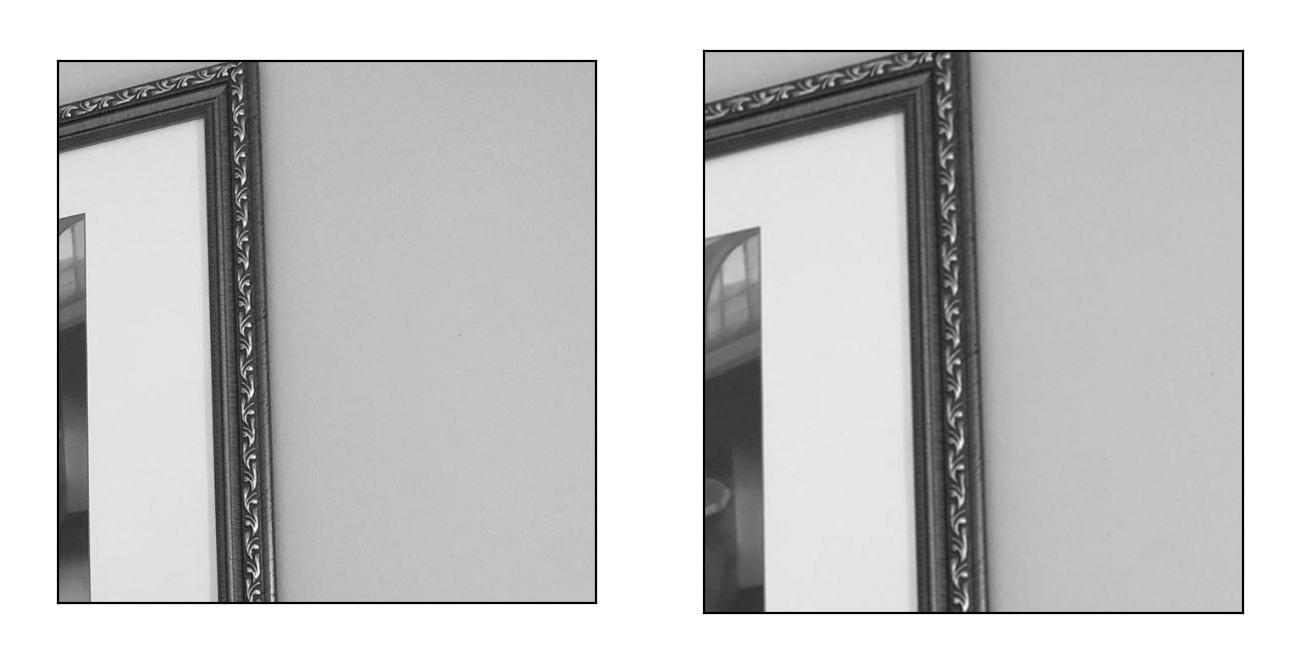
\includegraphics[width=.45\textheight]{fig1.png}
	\caption{Raw Image Pattern (LHS) versus Gaussian Blur Pattern (RHS)}
	\label{fig:001}
\end{figure}
\\
In Figure \ref{fig:001}, we use $3\times 3$ Gaussian Filter with standard devation $10$ to smooth the image. It can be observed that, in the LHS, the image is more clear and in the RHS, the image is more blur. Moreover, in LHS, the edge is shaper due to the complicated pattern in photo frame.
\vspace{4pt}
\\
Actually the complex pattern in image is not a good thing for image processing, since it will make the image gradient unstable. As a consequence, we will generate more useless edges which we are not interested in.
\vspace{4pt}
\\
To give an example, in Figure \ref{fig:001}, our interests can be the boundary of photo. However, if given complex patterns, then there are plenty of edges generated by complex patterns near the boundary, which will make the task more difficult. \textbf{This can be one motivation for us to choose Gaussian Filter}. Furthermore, the choice of filter size and corresponding std is critical, as we will show in the later discussion.
\subsection{Canny Detector}
One thing to discuss about Canny detector is, its choices of lower threshold and upper threshold. The mechanism of these 2 parameters is, if the magnitude of gradient is below $T_{low}$, then set the pixel value to 0. If the magnitude of gradient is above $T_{upper}$, then set it to 1 and marked as 'strong edge'. Otherwise, check whether this pixel is connected to one 'strong edge'. If so, set it to 1 and 0 instead. Noted that via Canny Detector, we can translate one gray image into bianry image, which can be used to find contours in the later stage.
\vspace{4pt}
\\
Therefore, if we want to remove those complicated patterns, we should set those 2 thresholds to be sufficiently large, such that we are able to filter them out. Notice that, this process can cooperate with different sizes of Gaussian Filter to extract features we want.
\vspace{4pt}
\\
Here, we use the previous example to illustrate the motivation. Observe that, there are plenty of thin edges between the inner and outer boundary of the painting. Based on this observation, it recommends us to use 'average' low-pass filter to smooth those thin edges, which is equivalent with Gaussian filter with large standard deviation. Here we choose $3\times 3$ Gaussian Filter with $std = 10$. Afterwards, to filter out those smoothed thin edges, we should choose a relatively big threshold. Here, we choose $T_{upper} = 300, T_{lower} = 100$. The final result can be shown in Figure \ref{fig:002}:
\begin{figure}[h]
	\centering
	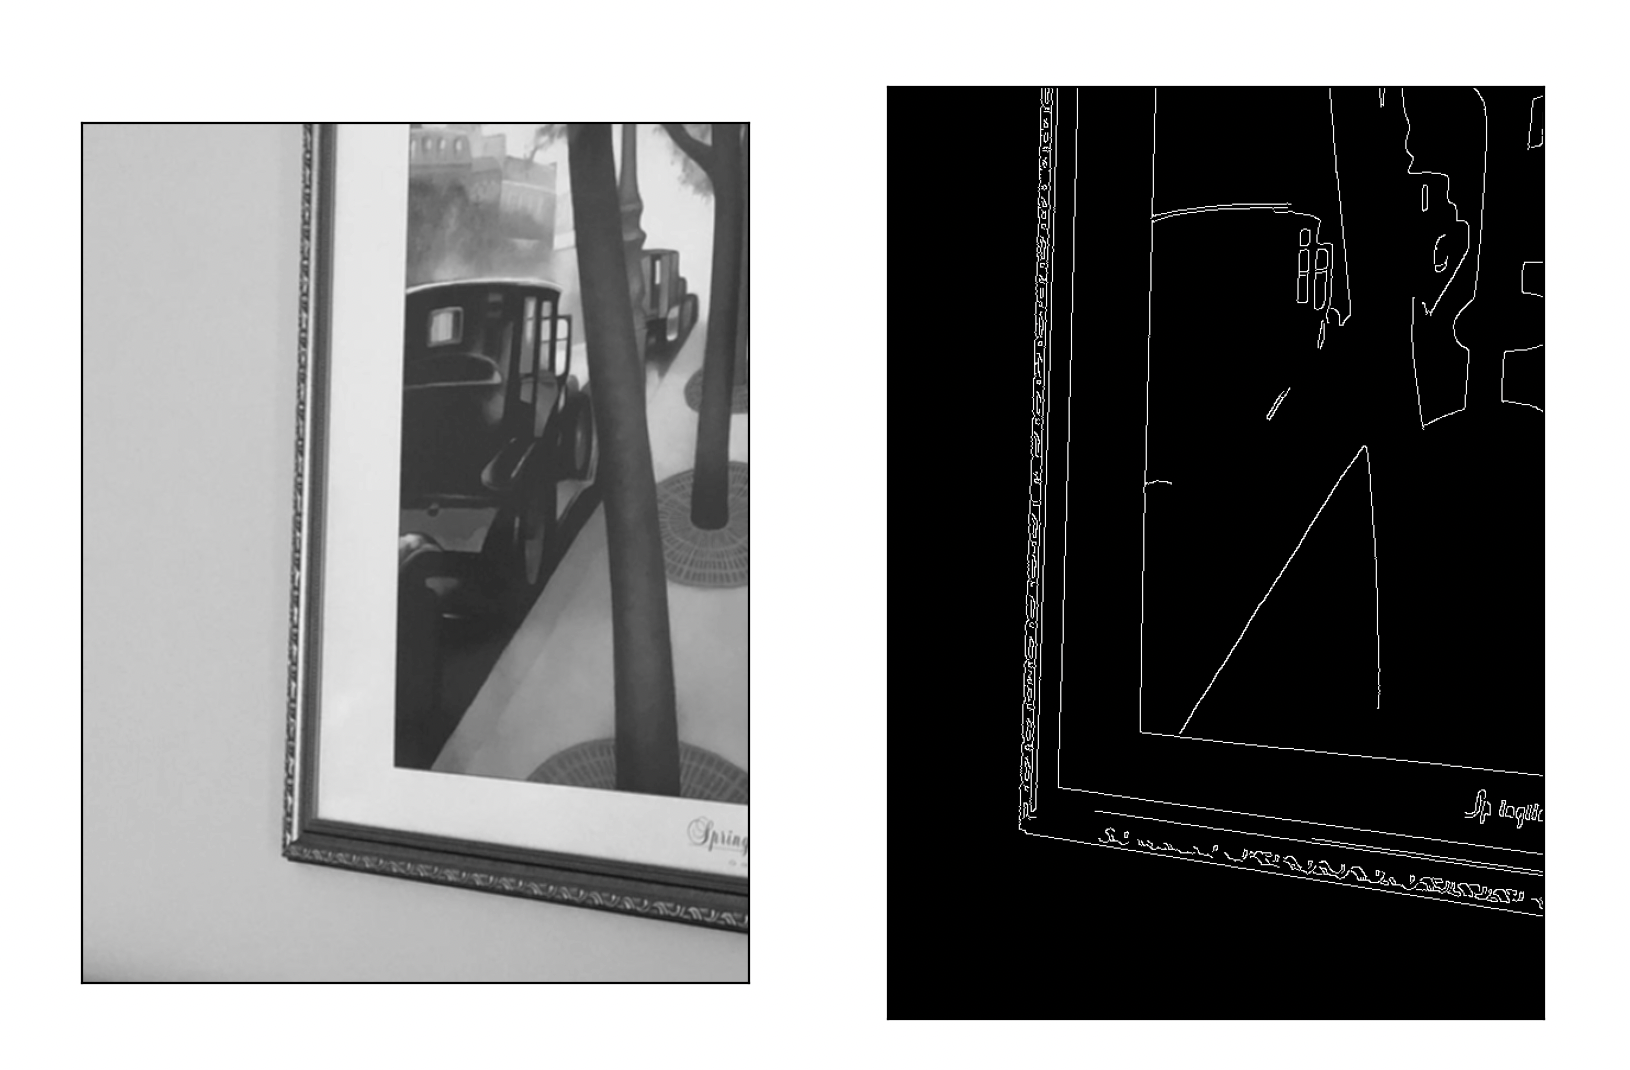
\includegraphics[width=.4\textheight]{fig2.png}
	\caption{Gassuain Blur and Canny Detector}
	\label{fig:002}
\end{figure}
\\
As you can see, the patterns between boundaries have already been smoothened. This makes the outer boundary smoother, which is approximately a line.
\vspace{4pt}
\\
To make comparison, if we use Gaussian Filter with small $std$ and Canny Detector with small threshold, then we will attain a more messy image. This can been shown as follows:
\begin{figure}[h]
	\centering
	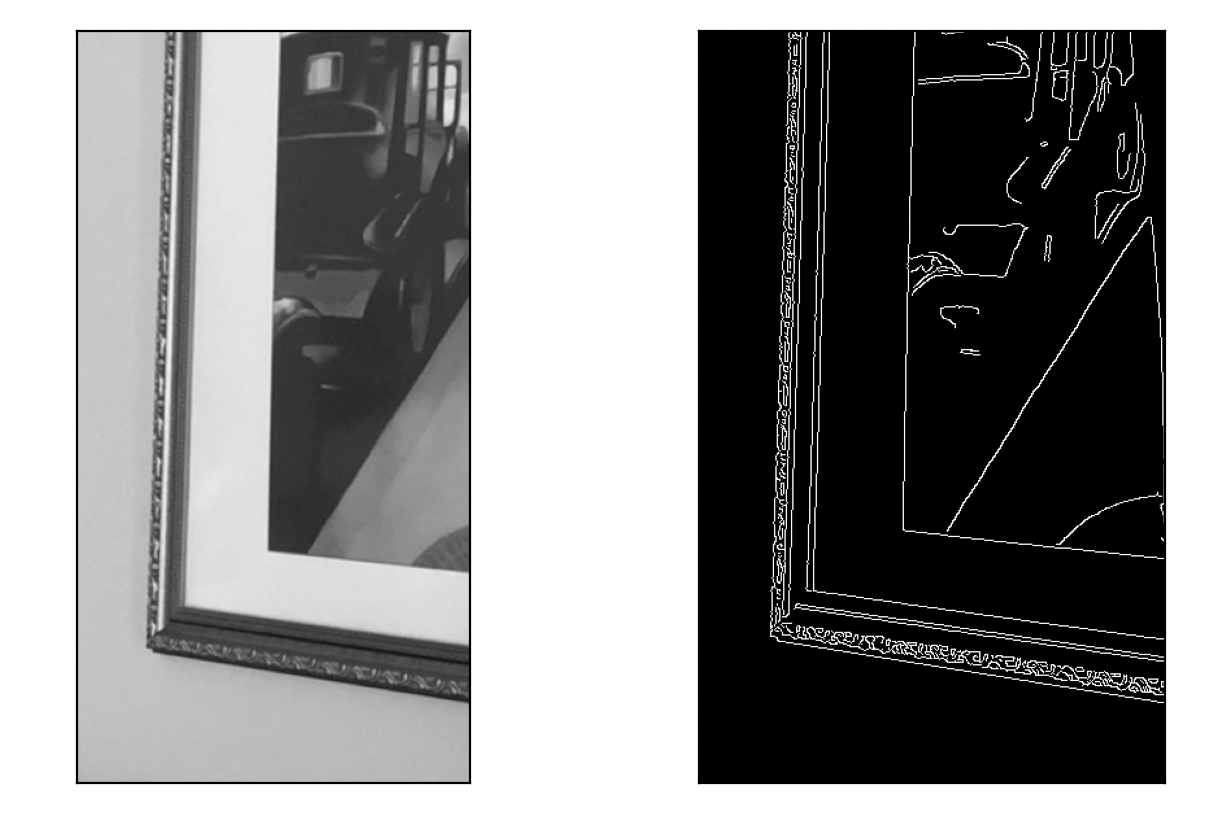
\includegraphics[width=.4\textheight]{fig3.png}
	\caption{Gassuain Blur and Canny Detector with small $std$}
	\label{fig:003}
\end{figure}
\\
In Figure \ref{fig:003}, you can easily observe that, there are more edges in the binary image generated by Canny Detector. That is, we preserve more detailed pattern of the raw image. This will bring great difficutly to detect contour since these detailed patterns can be viewed as noise with respect to the interested outer boundaries.
\newpage
\subsection{Contours}
After deriving those edges described by one binary image, we are abled to find contours via function pre-defined in cv2 package. This function actually returns all the contours. 
\vspace{4pt}
\\
In my application, I select the interested outer boundary via the largest-area contour. After that, find its 4 corner points, which will be used in perspective transformation fitting. Given utilize appropriate Gaussian Filter and Canny Detector (as shown in Figure \ref{fig:002}), the result of contours is shown as follows:
\begin{figure}[h]
	\centering
	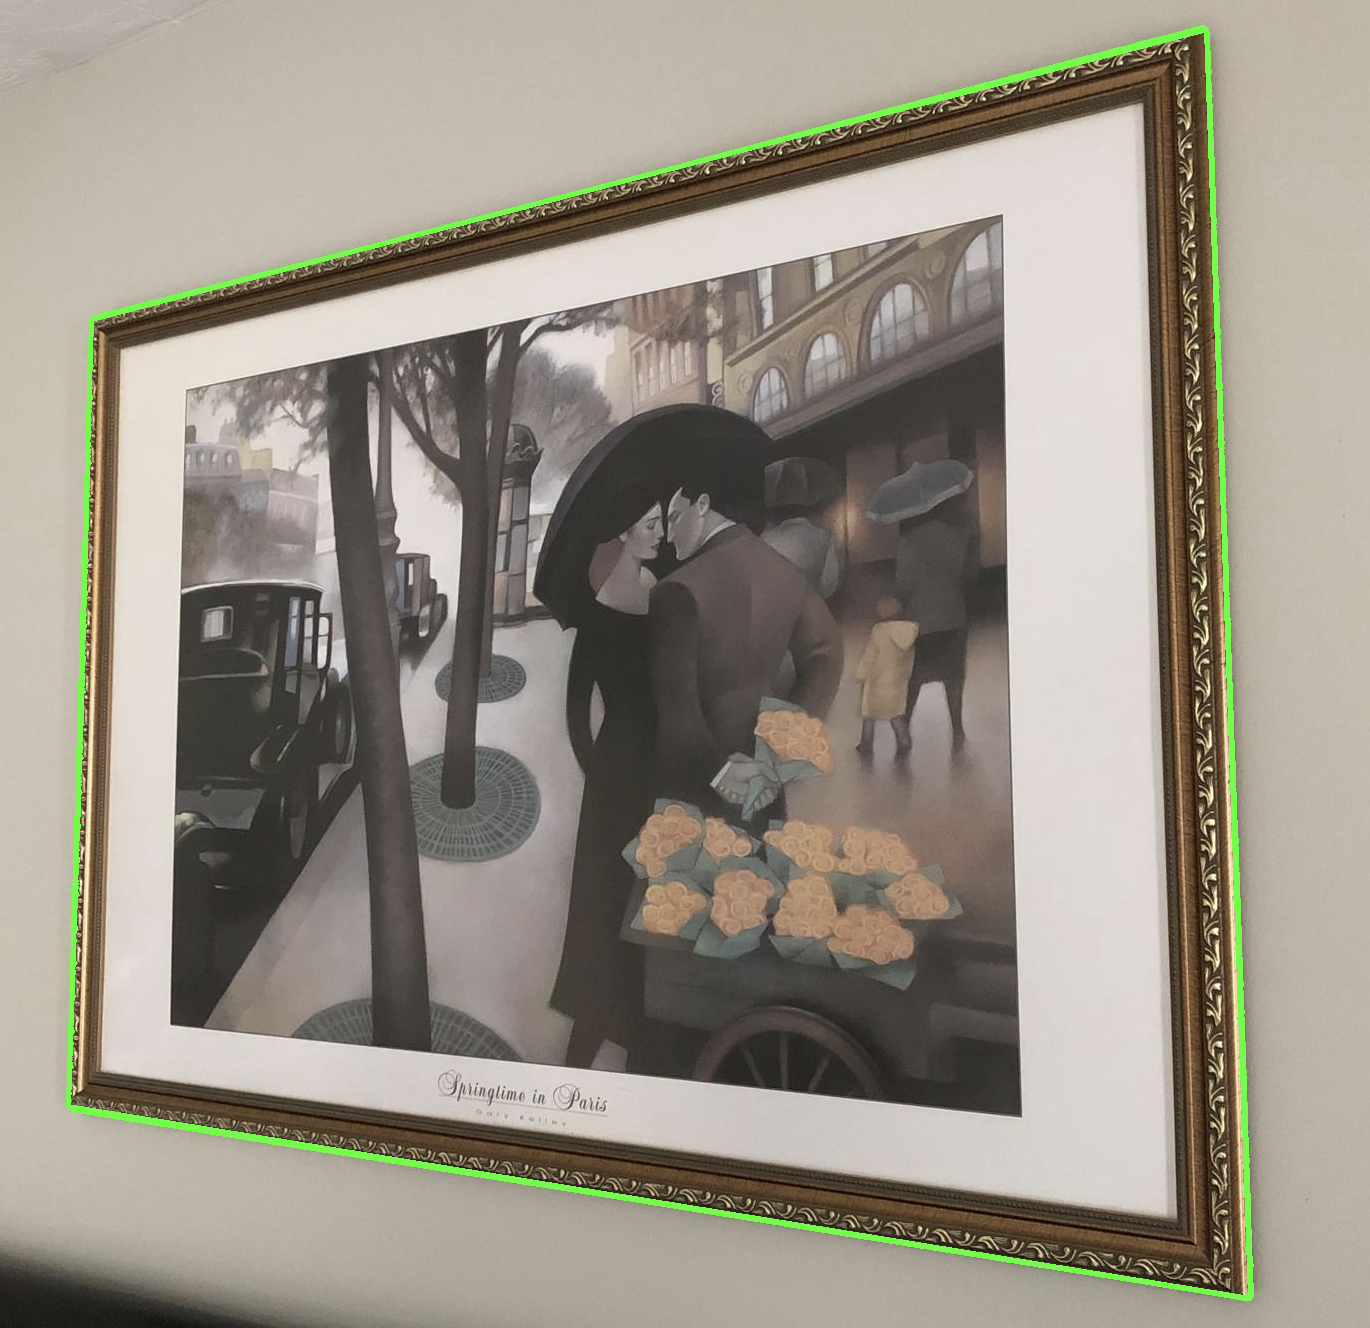
\includegraphics[width=.25\textheight]{fig4.png}
	\caption{Contours}
	\label{fig:004}
\end{figure}
\\
To make the algorithm more robust, we consider using the BINARY image via threshold for contour generation.
\subsection{Perspective Transfom}
After we attain the 4 corner points of outer boundary, we can fit for perspective tranformation matrix via Least Square Fitting.
\vspace{4pt}
\\
It is worthwhile to notice that, here we choose 'Perpsective Transformation' to approximate the rectified transformation. We do not choose affine transformation because in unrectified image, parallel lines will not be paralleled. We only want to guarantee the preservation of straight lines. This is why I use 'Perspective Transformation' instead of 'Affine Transformation' here. 
\vspace{4pt}
\\
Lastly, achieving the estimated perspective transformation, I warp the image via backward warping and the result is shown as follows:
\begin{figure}[h]
	\centering
	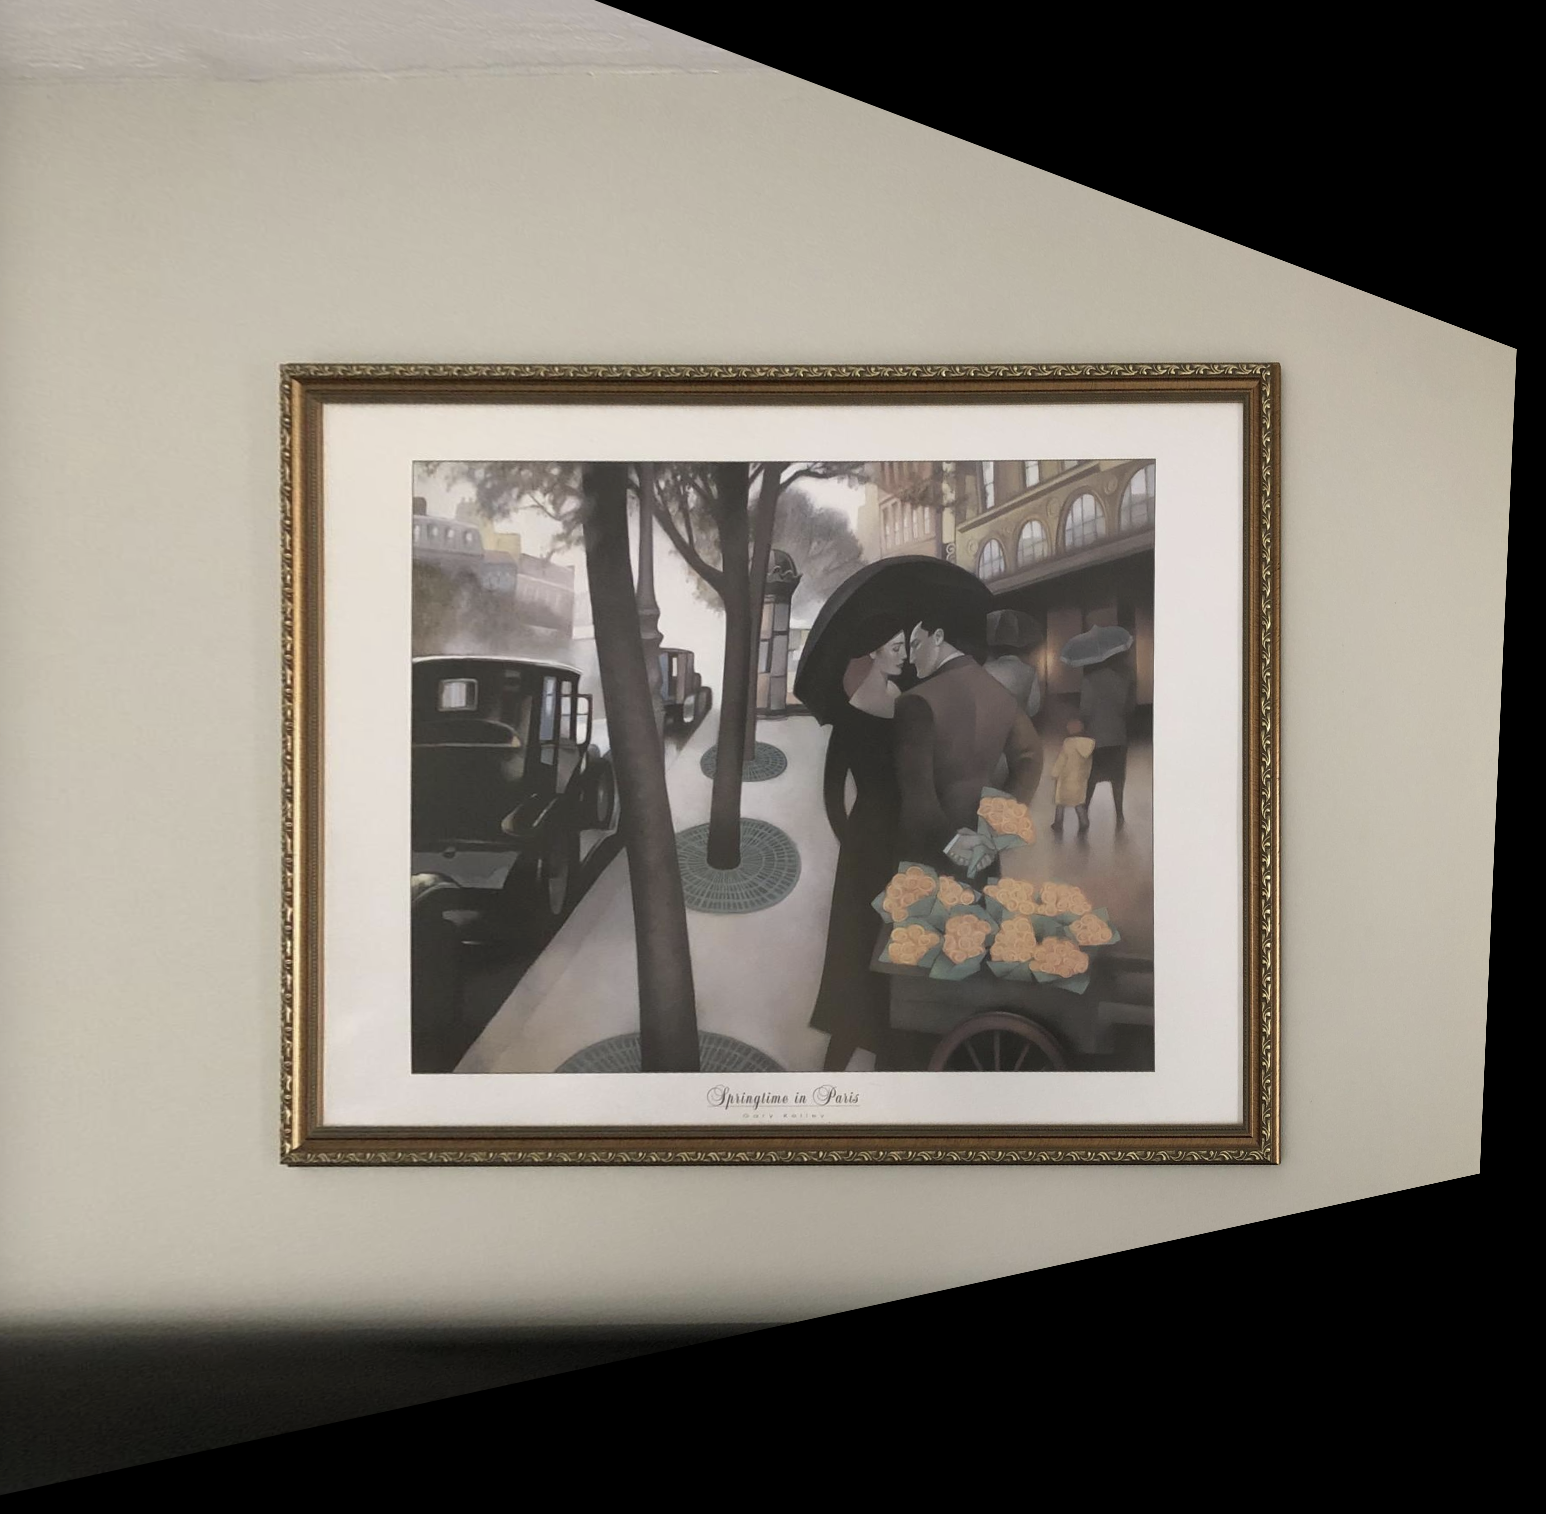
\includegraphics[width=.25\textheight]{fig5.png}
	\caption{Rectified image}
	\label{fig:005}
\end{figure}
\\
The result is pretty good!
\end{document}